\chapter{Discussion}
Our goal for conducting these studies were the following: \textit{Our goal for this study is to investigate the outcome returned from the retrospective in terms of organizational learning and retrospective characteristics.} Throughout this chapter we will first provide a descriptive discussion on the retrospective characteristics we have observed and then discuss the results in terms of organizational learning. Finally we will provide some reflections on the retrospective practice, the current state, a method proposal and some guidelines for conducting retrospectives. 

\section{Retrospective Characteristics}
One of our research objectives were: \textit{What are the main characteristics in current retrospective practices, in
terms of outcome, processes and impediments?} Throughout this section we will provide a descriptive discussion on the characteristics we have identified throughout our studies. The section is split into three parts: Output, Process Characteristics and Impediments. An overview of all the characteristics can be seen in \autoref{table:retrospective-properties}

\begin{table}[h]
	\begin{center}
		\caption{Retrospective characteristics}
		\label{table:retrospective-properties}
		\begin{tabular}{p{0.9\textwidth}}
			\hline
			\textit{Retrospective Characteristics}\\
			\hline
			\textbf{Output} \\
			Reflection on work processes, technical issues, work environment \\
			Creates improvement opportunities \\
			Improvement Implementation \\
			Provides organizational learning \\
			Improves shared mental model\\
			Can improve team enthusiasm \\
			Can decrease team enthusiasm \\ 
			Can improve efficiency  \\
			Facilitates empowerment \\
			\hline 
			\textbf{Process Characteristics}\\
			Little Considerations Taken \\
			Wish to Improve \\
			Varying techniques\\
			Occurs regularly\\
			Collects opinions from participants\\
			Arena for open discussion \\
			Allows for experiments in work environment\\
			Shared Learning Event\\
			\hline
			\textbf{Impediments}\\
			Team commitment\\
			Enforcing of process improvement actions\\
			\hline
		\end{tabular}
	\end{center}
\end{table}

\subsection{Output}
In this section we discuss the observations regarding the output of a retrospective process. The section is divided into ``Work areas'', ``improvements'' and ``Enthusiasm''. Some of these sections are divided into subsections, where we discuss relevant observations.

\subsubsection{Work areas}

Several work areas are covered by the retrospective. Mainly we have seen three areas that are covered by the retrospective. These areas are work processes, technical issues and issues related to the work environments. As we saw in team Zulu about 40\% of the actions created were related to technical issues and 59\% to process issues. Some of these issues might have been work environment related, however our content analysis did not include this. For future work this should be considered. From the interview with team Echo we learned that the team mostly discussed work environment issues as the team consisted of several sub-teams that worked differently from each other. 

We have seen very little of personnel issues brought up during the retrospective. Only case was with team Delta where one of the members never got help from the others. In team Zulu we saw that not being able to take up personnel issues hindered the retrospective. When asked several of the study participants voiced an opinion that personnel issues were something that should be taken outside of the retrospective to hinder blaming and a negative mood during the meeting. We have not seen any earlier literature discussing the topic. We do believe however that the consideration of including personnel issues is something that could be appended to Dingsøyr's \cite{Dingsoyr2004} set of considerations which should occur before the retrospective.

\subsubsection{Improvements}
Here we discuss the improvement outputs from a retrospective process. The outputs discussed are ``Creates Improvement Opportunities'', ``Improvement Implementation`'', ``Improves Shared Mental Model'' and ``Shared mental models practice`''. 

\paragraph{Creates Improvement Opportunities}
Through our studies we have seen that teams are able to improve based on decisions created during the retrospective. From the depth study of Team Zulu's we saw that through 77 retrospectives the team had created 343 actions which reflects improvement opportunities. Also all the teams in our breadth study created actions to improve some aspect of their work-life. It is clearly evidence that improvement opportunities are created through the retrospective. This seems to fit well with previous \cite{Larsen2006, Dingsoyr2004, Drury2012} that the retrospective help identify improvement opportunities. 

\paragraph{Improvement Implementation}
The question if the improvement opportunities are actually implemented can also be seen through our studies. The results of our studies revealed that most of the teams were satisfied with their implementation rate. From team Zulu we learned that only 65 of the 343 actions were not yet implemented. It was also revealed that implementation could be a challenge, as was the case with Team Charlie. We identified two methods that seemed to help overcome this challenge. The first was assigning responsible team members to each action. The second was SCRUM master follow-up of the actions. We have seen that retrospective practicing agile development teams are able to implement improvement opportunities confirming Derby and Larsen's \cite{Larsen2006} statement of retrospective helping team adapt and contradicting the research of Drury et. al. \cite{Drury2012} which finds that no real changes occur as a result of the retrospective. 

\paragraph{Improves Shared Mental Model}
The knowing stage is not included in the domain of the sprint retrospective described by Petter et al. \cite{Petter2013}, in our work we found that the facet of team members sharing their individual knowledge, thereby updating the shared information. One example of this was found in team Echo, where the different sub teams would use the retrospective to share their discoveries and knowledge development, thus updating the meta-knowledge of the team as a whole. 

The learning phase of the shared mental model and is impacted by the agile retrospective by using techniques that facilitate the integration of the knowledge from the knowing stage. One example could be the use of evidence based time lines as described by Bjarnasson et al. \cite{Bjarnason2012}, where the time line would work as an outline of the information received by the team. Another example is seen in the weekly retrospectives held by team Alfa, where team members would continually update their colleagues on their work day, allowing for reflexivity. Another example would be the use of the ``five times why'' as used by team Charlie and Echo, where both the possibility for reflexivity and self correction exists.

The understanding phase described by Petter et al. \cite{Petter2013} is far reaching and includes many facets of team cooperation and some of them are described in \autoref{section:mental-models-stages}. One part of the understanding phase we did not expect to see explicitly in our study was conflict resolution on a personnel level, and can be considered part of the conflict reconciliation and consensus building that is part of the understanding phase. Also part of the understanding phase is the practice of refining team communication and team processes which is a central component of the retrospective purpose, and we observed every team discussing these topic during our interviews and analysis. Lastly, not included in the work of Petter et al. is the use of the retrospective as a tool for planing, and 24.6 percent of the actions analyzed in our work with team Zulu were deemed to have a planning component, as described in \autoref{section:development-phase}. This planning component could be said to be increasing the similarity of the information between team members.

The execution is perhaps the phase most impacted by the retrospective, as the explicit actions decided during a retrospective almost always is intended to improve or refine the processes that in one way or another help the reach their goals. For example the information similarity generated in the understanding phase can lead to a quicker response time to new tasks. One typical example is the refining of the communication processes as seen in team Zulu, or the introduction of the bug-fix days described in \autoref{section:bugfix}. 

\paragraph{Shared mental models practice}
In this section we discuss observations on the relationship between retrospectives and shared mental model practices.

Reflectivity is a central part of the learning process in the team. We have observed that many teams use the retrospective as a review tool of the last work period. We have observer very different practices when it comes to frequency as seen in \autoref{table:frequency-duration}, and thus the definition of a work period is different from the sprint retrospective definition from Peter et al. One observation done by us is that very few teams practice reflectivity on the retrospective itself, or if they do they do not formally do it on the team level, as seen in team Charlie. In team Charlie the scrum master would discuss and reflect on the retrospective with other scrum masters and team leaders within the company, but it would not be brought back to the team. In some ways the analysis done with team Zulu together with the feedback sessions with them could potentially be considered an example of this kind of reflectivity. The interviews done with team Zulu's leader and scrum master suggests that both the team's mental model similarity and accuracy was improved through the analysis and reflection done, this is described in \autoref{section:feedback-session 4}

The sprint retrospective defined by Petter et al. Does not include planning, but our work with team Zulu indicates that planning is an integral part of retrospective actions in some teams. This is discussed in \autoref{section:development-phase}, this high degree of presence of planning was unexpected and more thought on the potential of mental model improvement through planning in retrospective seems interesting. For example the use consensus based approach used by team Golf in planning could potentially increase the similarity of the team's mental model.

\paragraph{Can Improve Efficiency}
The retrospective practice can, as we have seen in multiple examples, improve the efficiency of teams conducting them. Team Echo's practice changes from SCRUM to KANBAN and then to modified SCRUM and Team Zulu's ``Bug-crunch day'' is just two of the examples we have seen that the teams have been able to improve their efficiency through the retrospective practice. This again confirms the previous literature \cite{Dingsoyr2004, Larsen2006, Kinoshita2008} that retrospective are able to improve practices and contradicts the finding of Drury et. al. \cite{Drury2012} that retrospectives provides no real changes.

\subsubsection{Enthusiasm}
\label{section:positive-loop-enthusiasm}
Team enthusiasm is both affected the retrospective practice and inflicted by it. It can be increased through a positive feedback loop or decreased by a negative feedback loop. As a result of the retrospective practice individual empowerment is facilitated and this also increases the enthusiasm. We will describe and discuss each of these statements below through examples from our studies and earlier literature. 

\paragraph{Can Improve Team Enthusiasm}
We seen that the enthusiasm of the participants of retrospective practice can be both affected by the retrospective. We uncovered a positive loop that helps increase the enthusiasm of the team conducting retrospectives. If changes occurred as a result of the retrospective the participants would become enthusiastic and thus the chance of more changes would occur. Ownership towards the development process was one factor that could help increase the enthusiasm and feed the positive loop. The positive loop confirms what Derby and Larsen \cite{Larsen2006} states that teams are invested in the success of improving their work as the improvements are chosen by the teams themselves and not from upper management. 

\paragraph{Can Decrease Team Enthusiasm}
The retrospective practice has also the ability to decrease the enthusiasm of the practicing team. As the opposite of the positive loop a negative are able to decrease the enthusiasm. If no changes occur enthusiasm will decrease and as the enthusiasm decreases the chance of new changes occurring decreases. Some even might see the retrospective as a waste of time as described by team Charlie's SCRUM master which had happened with some of the teams in his department. This confirms our previous literature review \cite{Dolvik2014} that recurring issues kills the joy and Drury et. al. \cite{Drury2012} that some may see the retrospective as a waste of time. 

\paragraph{Facilitates Empowerment}
Ownership towards the development process was seen as crucial towards getting improvement out of the retrospective by the interviewed teams. Each team member has the possibility to participate in shaping their working process through the retrospective. As seen in team Alfa and Echo even the shy are required to participate in returning feedback and contribute solutions for current work processes. Tessem \cite{Tessem2014} identifies participation in process improvements as an empowering practice. This directly relates to the retrospective practice, which is also a parallel drawn by Tessem and we now confirm. Enthusiasm is increased as members are empowered\cite{Tessem2014} and thus the retrospective increase enthusiasm through empowerment. 

\subsection{Processes Characteristics}
In this subsection we will discuss the process characteristics observations we made in relation to our results and established theory. The subsection will be divided into before, during and after.

\subsubsection{Before}
As seen in \autoref{section:Dingsoyr-Approach-Introduction} we will compare our observation results of the work done before a retrospective primarily to the theory from Dingsøyr's ~\cite{Dingsoyr2004} work. This section is divided into ``Little Considerations Taken'', ``Wish to Improve'' and ``Facilitator''.

\paragraph{Little Considerations Taken}
When we consider our results we see that few of the teams interviewed do a thorough consideration of their practices in relation to the approaches seen in \autoref{table:postmortem-approach}. Most teams did not do a informed decision on several Dingsøyr's considerations. For example on who to invite or sharing tacit and explicit knowledge. For example team Alpha's interviewee said that it could go long periods of time where a developer was not invited to a retrospective. When it comes to sharing the knowledge generated none of the teams made a concerted to share the knowledge that came as a results of learning through the retrospective.

\paragraph{Wish to Improve}
Many teams had a great wish to improve. As seen throughout our results the need to build a culture that allows for learning is absolutely essential for a productive environment, this is in accord with  Dingsøyr's work. Especially trust between the team members emerged as critical for reaching the maximum potential of a retrospective session. An example of the possible improvements is the team dynamic improvements experienced by team Delta when one of their team members brought up the problem that he was not getting help from other team members, as described in \autoref{question-21}. Also after our depth analysis with team Zulu their eagerness to improve let them turn the results from our analysis into a basis for multiple actions intended to improve the team's learning capabilities. 

\paragraph{Facilitator}
\label{section:facilitator}
Deciding on the facilitator can be considered both part of before the retrospective, and during. As work needs to be done in advance and Few teams used an external facilitator as recommended and the experiences we observed were uniformly positive. This is in accord with Dingsøyr's work. However only two teams used external facilitators consistently, as described in \autoref{question-12}. Team Zulu had only one experience with using an external facilitator but it was described as a very productive and positive experience. Perhaps this indicates that many teams would benefit from making a more concerted effort to utilize external facilitators. 


\subsubsection{During}
In this section we will discuss our observations relating to what happens during the retrospective process. This is divided into ``Occurs Regularly'', ``Collects Opinions from Participants'' and ``Open Arena for Discussion''.

\paragraph{Occurs Regularly}
Retrospectives happens at a regular basis varying from team to team from every week to every six months. Usually it occurs after an ending of a development stage either a project iteration or a released feature.

\paragraph{Collects Opinions from Participants}
During the retrospective data is gathered from the participants. We have seen that feelings and opinions are two primary data types gathered. None of the teams in this study have used other sources of data for their retrospective, with one exception of lead times which were used by one of the teams. The participants in the retrospective consists of team members contributing to a project iteration or feature that the retrospective focuses on. These consists of developers, testers, designers, architects,consultants, SCRUM masters and in some cases project leaders as seen in Team Zulu. 

\paragraph{Open Arena for Discussion}
The retrospective provides an open arena for discussion. Each participant are allowed to bring their own issues and the issues are then analyzed through discussion or root-cause analysis. An facilitator, either internal from team or external, facilitates the discussion. From the facilitators we have spoken to some censor the discussion on some subjects. In team Alfa personnel cases where not allowed and would have to be discussed outside the retrospective. In team Delta the SCRUM master tried to hinder technical discussions as their focus is on work processes. Other than this most topics are allowed during the retrospective as we have seen in Team Zulu. Through our depth study we saw that.

\subsubsection{After}
In this section is our discussion on factors that take place after the retrospective process. This is divided into ``Allows for Experiments in the Work Place'' and ``Shared Learning Event''. 

\paragraph{Allows for Experiments in the Work Place}
\label{section:experiments-in-work-place}
As seen in \autoref{section:Derby-Larsen-Structure} a retrospective can be an area that facilitates experimentation in a team. We have observed this, for example as described with team Echo in section \autoref{question-11}. Here team Echo tried to move to KANBAN from SCRUM, the experiment was not an immediate success, but allowed them to return to a SCRUM methodology that they could tailor after their experiences from the experiment. This resulted in their work methodology fitting their team better. Our work with team Zulu also led to experimentation, for example their decision to create a dashboard to log their retrospective actions. Another experiment by team Zulu was the inclusion of a ``bug-crunch'' day seen in \autoref{question-11}. This experiment was a success and led to a noticeable decrease in bugs.

\paragraph{Shared Learning Event}
The theory of the retrospective as a shared learning event was described in \autoref{intro:retro-outcome}.  An example of a shared learning event from the same section was performed by team Delta, as they changed their time estimation practices to great success after discussing the process in a retrospective. However none of the teams interviewed made an organized effort to make the result of the retrospective a learning event for personnel outside the team, as mentioned by Dingsøyr ~\cite{Dingsoyr2004}.



\subsection{Impediments}
In this section we discuss our observations on impediments in context of the retrospective process. The sections is divided into ``Personalities'', ``Team Commitment'', ``Enforcing of Process Improvement Actions'' and ``Availability''.

\paragraph{Personalities}
Some personalities could provide obstacles for the retrospective. We saw three examples of this. The first one was in Team Zulu where cultural differences provided miscommunication and difficulty providing an open discussion in the retrospective. The second was in the department to team Charlie where some SCRUM masters had low enthusiasm for the retrospective practice and this could influence the rest of the teams as well. The third example were two senior developers with strong personalities, in team Charlie, that could hinder the other developers from voicing their opinions. These were the only three cases we saw in our studies, but further personalities may be investigated. Derby and Larsen \cite{Larsen2006} talks about personalities that take a lot of time and hinder others from taking part in the retrospective and this is reflected pretty well in the last example. They suggest that talking to them privately and directly asking them to hold back a little could help the situation. Team Alfa recommended using KJ-sessions to help everyone participate.

\paragraph{Team Commitment}
Even though most of the teams in our study was satisfied with the commitment from their teams, implementation of actions still could provide a challenge. As mentioned by several of the interviewees if the actions were not assigned to a specific person the action would not be implemented. This indicates that the team as a whole don't have the commitment to implementation of retrospective actions. Drury et. al. \cite{Drury2012} described several obstacles that it fits with these results. Team members unwilling to commit and relying on SCRUM master, not implementing decisions or relying on others for decisions, and not taking ownership of decisions are all obstacles that could be identified through our research. However as mentioned this was only the case when the group as whole was assigned to a decision, when individuals of the group were assigned the teams were satisfied with the implementation rate. This still indicates however a lack of team commitment even though the consequences are dealt with. 

\paragraph{Enforcing of Process Improvement Actions}
Enforcing the implementation of process improvement actions were seen as a challenge. The SCRUM master of team Zulu described how enforcing and monitoring process improvement actions was a challenge. Some process changes required the whole team to implement the action and both enforcing the implementation and monitor it could be hard. Conflicting priorities and not taking ownership for decisions are two of Drury's et. al. \cite{Drury2012} obstacles to effective decision making, and these results reflects the two obstacles. 

\paragraph{Availability}
The last impediment we have seen for conducting retrospective is availability. In team Golf we saw how having a distributed team could make it harder to conduct the retrospective. In team Alfa and Foxtrot we learned how the unavailability of retrospective due to long timespan or participants not being able to participate could inhibit the retrospective. Zedtwitz's \cite{Zedtwitz2002} barrier of memory bias and Drury et. al. \cite{Drury2012} obstacle of unavailable staff is reflected in this. 

\clearpage

\section{Organizational Learning} % (fold)
One of our research objectives were: \textit{How is learning achieved through current retrospective practices, in light of organizational learning theory?} Throughout this section we will first discuss the results of our case-studies in terms of the governing values of Argyris and Schön's \cite{Argyris1996} organizational learning Model I and Model II. Secondly we will discuss our results in terms of learning types. Finally we will discuss the impediments for learning that we have seen throughout our studies. 

\label{sec:organizational_learning}
\subsection{Governing Values}
Argyris and Schön\cite{Argyris1996} described several governing values for learning organizations as we described in \autoref{intro:organizational-learning}. Throughout this section we will reflect on our results using these governing values investigating how retrospectives is performing as a learning practice. 

\subsubsection{Model I}
In Model I, described in \autoref{sub:model_i}, four governing values set the focus for the learning organization. Into our investigation of the retrospective practice we have seen very little to any of these values. We will discuss this below for each governing value and then the consequences before we summaries the findings related to Model I.  

\paragraph{Setting and  Achieving Goals}
One could argue that the team setting goals and achieving them could be compared to creating actions and fulfilling them, however we do not support this as the fulfillment of actions is part of a collective efficiency improvement and learning practice. The retrospective and its participants are instead of trying to design and manage the environment unilaterally, investigating all the different angles and perspective the team can present and finding solutions to the problems existing within that environment. The joint team discussion and retrospective practices are evidence of this. 

\paragraph{Maximize Winning and Minimize Losing}
Maximizing winning and minimizing loosing is not visual in the current retrospective practice. The teams are not afraid to use the retrospective as an arena for creating experiments on new practices where some might work and some might not. Team Delta and Echo, gave examples where the teams had tried to implement new practices and instead of going down with ship when the practice had not worked, leave ship and try something else. In Team Delta things that did not work for the members of the team simply did not get done and it was a joint understanding that actions that did not get any attention were bad practices. In Team Echo the team was not satisfied with current work practices and changed them drastically. After some months time they found that these new practices only made thing worse and instead of claiming ownership for the task and try to force it through the team decided to try something new. 

\paragraph{Minimize Generating or Expressing Negative Feelings}
Through retrospectives we have seen that the participants are allowed to express their feelings regardless of their good or bad. This effectively counter the third governing value which is minimizing generating or expressing negative feelings. Team Echo and Delta both described events that showed participants raising negative issues and feelings towards the team. From the retrospective analysis for Team Zulu we saw that 89.3\% of the actions created came from negative issues. Even though allowing negative feelings are good thing some of the interview subjects said it could become a little bit to much negative sometimes, and that the retrospective is not a arena to vent. As was the case with Team Zulu the third and fourth feedback session revealed that the team had become more aware of raising also good feelings and issues during the retrospective and such they felt the retrospective had improved. This indicates that allowing negative feelings is important as one can learn and improve from them. However one should also ensure that good feelings are raised as they also provides the same opportunities and creates a more enthusiastic feeling about the retrospective.

\paragraph{Be Rational}
As feelings are encouraged to share during the retrospective, to some moderation, the fourth governing value being rational also seemed to not be the apparent in the retrospective. Being rational implies censoring feelings and as we described above retrospectives encourages sharing of feelings towards the group. 

\paragraph{Consequences}
The consequences resulting from Model I governing values also seems to be rarely encountered in retrospectives in terms of the behavior. We have witnessed one case where an actor acted defensibly and such created an atmosphere that suppressed the other participants feelings. Creating what was described in an elephant in the room. It was also confirmed by the interviews that personnel issues were not addressed during the retrospective and such events could decrease the value gained from the retrospective. Other than this we have neither seen or heard about teams having defensive norms, or having defensive interpersonal relationships. 

Most of the learning consequences seems to be opposite of what is expected by Model I except single-loop learning and possibly decreased long-term effectiveness. It might not be that surprising that as the governing values are rarely encountered that the consequences of them is not either. Neither self-sealing, lack of public testing of theory or too much testing of theory in private seems to be appearing in teams conducting retrospectives. What is more surprising is that single-loop is quite occurring. We will dwell deeper into this in \autoref{discussion:learning-types}. In terms of decreased effectiveness we have no way compare these to any of our results as we lack a control group applying most of the governing values from Model I. 

\paragraph{Model I Summary}
The governing values from Argyris and Schön's Model I seems to not occur or be the system employed by agile development teams performing retrospective systems today. We have only seen two cases where the governing values of Model I has had any implications on the team. The first one was that of face-saving from one of the team members resulting in an atmosphere suppressing the other members feelings. This member later left the team. The other implications of Model I governing values is that of single-loop learning which most teams experience and will be discussed further in \autoref{discussion:learning-types}

\begin{table}[h]
	\begin{center}
		\caption{Governing values and consequences encountered in relation to retrospectives.}
		\label{table:model-i-occurences}
		\begin{tabular}{l l}
			\hline
			\textit{Model I} & \textit{Encountered} \\
			\hline
			\textbf{Governing Values} & \\
			Defined goals and try to achieve them. & No \\
			Maximize winning and minimize loosing. & No \\
			Minimize generating or expressing negative feelings & No \\
			Be rational & No \\
			\hline
			\textbf{Behavioral World Consequences} & \\
			Defensive Actors & Once observed \\
			Defensive Interpersonal and group relationship & No \\
			Defensive Norms & No \\
			\hline
			\textbf{Learning Consequences} & \\
			Self-sealing & No \\
			Decreased long-term effectiveness & Not observed \\
			Single-loop learning & Yes \\
			Little testing of theories publicly & No \\
			Much testing of theories privately & No \\
			\hline
		\end{tabular}
	\end{center}
\end{table}

\subsubsection{Model II}
The governing values of Argyris and Schön's Model II are more apparent in the teams that practice retrospectives. We will discuss our findings related to each of the governing values and the consequences observed below. A summary of this discussion is at the end of the subsection. 

\paragraph{Valid Information}
\label{section:valid-information}
Valid information is the first of the governing values of Model II and the retrospective practice require information gathering from the team members. We have seen several ways that retrospective teams gathered information. Nominal brainstorming through KJ-session, around the table discussion and others techniques have all been used to gather information and finding issues with the development process. Zedtwitz\cite{Zedtwitz2002} found memory bias as one of the barriers to learning and Bjarnason and Regnell\cite{Bjarnason2012} proposed evidence based timelines as a technique to counter this. None of the teams we investigated used this technique and none of them mentioned memory bias being a problem for the retrospective. Neither did we see this through our content analysis of Team Zulu. However during the feedback sessions with team Zulu looking back at specific events happening a year past the team was uncertain. This gives us reason to believe that in terms of iteration retrospective which happen regularly with a timespan of weeks don't suffer from memory bias. However feature driven retrospectives and project retrospectives could suffer from this. 

To identify the issues we have seen that the practitioners of retrospectives uses only information gathered from the participants with one exception of a team using lead times as a measurement tool. However we have not seen many examples on using other information tools to evaluate solutions for issues than the participants of the meeting. We have seen team Zulu and team Foxtrot postponing issues until they can investigate it further. This have not come up in our discussions with other teams, but it can seem that the teams during retrospectives acquire knowledge when their own is lacking.

\paragraph{Free and Informed Choice}
The second governing value of Model II is free and informed choice and through our study we have seen that teams are mostly free to make their own improvements through the retrospective. Many firms have adopted agile methodologies and an important part of it is having short feedback loops and thus the retrospective can be a valuable practice. None of the teams spoke of problems with management having too little time or being allowed to conduct retrospective. This effectively eliminates Zedtwitz\cite{Zedtwitz2002} barrier of managerial time-constraints. The second managerial barrier of bureaucratic overhead is also for most cases absent from the retrospective practice. Teams are free to conduct the retrospectives in any matter they themselves chooses. The only cases where the barrier provide any impediments is cases where implementing an action has a high resource cost which we learned form Team Alfa. Also issues that required change with external parties could hinder implementation as we learned form Team Zulu. Other than that we seen that all the teams are free to conduct and manage their own retrospective practice, providing an environment of free and informed choice for the team. 

\paragraph{Internal Commitment to the Choice and Constant Monitoring of its Implementation}
The third and final governing value of Argyris and Schön's Model II for organizational learning is internal commitment to the choice and constant monitoring of its implementation. This value is one of the challenges facing retrospectives today. All the teams in the study emphasized that getting things done and actually see the actions followed through was crucial to having a valuable retrospective. If the team could not see any choices become implemented this would create a negative feedback loop where participants enthusiasm would lower and the chance of new actions being implemented would decrease even further. However as we have seen in our content analysis only 19\% of the actions created was still left unresolved. Most of the other teams we interviewed seemed pleased with the action implementation. That most teams acknowledged the risk of not implementing actions reveals that teams have a focus towards maintaining the issue. 

Enforcing process improvements was admitted as a challenge by some of the teams and thus reveals that implementation of actions could prove difficult. Considering all the input we got on the subject push-tactics, assigning responsible individual, worked better than pull-tactic where it was expected that some would handle the implementation. This reveals a lack of commitment and aligns well with Drury et. al. \cite{Drury2012} findings that daily operational tasks triumphs that of strategic/tactical tasks found during the retrospective. The interviews revealed that enabling the team-members to acquire an ownership towards the work process improved the commitment to the retrospective and implementation of tasks. Some teams also added retrospective actions as a part of backlog to increase the implementation rate. 

\paragraph{Consequences}
The consequences of the three governing values for Model II are both apparent and absent in the teams participating in the study.

According to Model II, organizations that focuses toward an organizational learning II system will have actors that are experienced as minimally defensive. As earlier mentioned we seen only one case were an actor has behaved defensively, and where the actor later left. The retrospective practice would suffer during such actors as seen in case of Team Zulu, censoring the rest of the team as they would not openly give blame to the actor. Reluctance to blame is one of the team base barriers identified by Zedtwitz\cite{Zedtwitz2002} and the team suffered for this. However as this was a single case it indicates that such types of actors are not welcomed into teams approaching such organizational learning II systems. Thus we can say that actors are minimally defensive during participation in retrospective. Zedtwitz barrier of blaming will also seem to be removed. However we have not seen any blaming during our studies and as earlier mentioned, \autoref{sub:model_i}, this is an action strategy occurring in organizational learning system applying Model I which one would seek to avoid. Instead replacing it with confrontation current views. 

Another consequences of the behavioral world, described by Argyris and Schön, is: ``Minimally defensive interpersonal relations and group dynamics''. In general our study has seen little of actors, that are participating in retrospectives, acting defensively towards the other participants in the group. We have only seen two examples that actors act defensively The first one in team Alfa where it was acknowledged that friction between some sensitive participants and some very outspoken could be a challenging at times. And in team Zulu where a foreign developer acted very defensively. In these cases the problems have been solved. Team Alfa said that experienced facilitators could lessen the friction and team Zulu removed the developer from the team. Team Delta provided an excellent example on one of the actors acting minimally defensive. The actor had acknowledged for the rest of the group that he wasn't able to get help from anyone. The SCRUM master said that trust had made it possible to bring up the issue. One can deduce that acting minimally defensive towards others is closely related to trusting one another. Team Alfa and Echo also said that trust was important for the retrospective. 

The retrospective in itself is a learning-oriented norm, which is the third consequence described by Model II. The participants of a retrospective performs it to learn from the last phase of a development process, and find new opportunities to improve. 

The fourth consequence of the behavioral world is related to freedom of choice, internal commitment and risk taking, which the retrospective all provide an opportunity for. As mentioned above the freedom of choice and risk taking are granted by the retrospective as long as it is not to costly in terms of resources or requires change from an external party to the retrospective team. Internal commitment can be, as described above, a challenge to agile teams performing retrospective, and creating ownership towards the development process as well as implementing actions is important to overcome this barrier.  

The consequences of learning and effectiveness for approaching a Model II learning system is frequent public testing of theories, double-loop learning and disconfirmable processes. 

Frequent public testing and disconrfirmable processes are both seen throughout our studies. Conducting retrospectives enforces participants inquiry into their current work processes and adapt, discard or improve them. An example of this is team Echo who changed practices from SCRUM to Kanban to improve, but found that this was less effective and instead went back to an adapted version of SCRUM that suited the team better. 

Double-loop learning on the other hand is not as apparent as the rest of the consequences and we will dwell more into this in \autoref{discussion:learning-types}. 

For the increased effectiveness the retrospective seems to yield better work practices. Most teams in our studies revealed that the retrospective helped increasing effectiveness for the work practices. 

\paragraph{Model II Summary}
The governing values and it's consequences for Argyris and Schön's Model II of organizational learning systems are both apparent and absent from agile teams and retrospective. Valid information and free and informed choice are both seen in retrospectives. Internal commitment and implementation is also seen, but regarded as a challenge by the teams conducting retrospective. The behavioral consequences this yields is relationships between actors and the actors themselves are less defensive, learning oriented norms and high freedom of choice and risk taking. The learning consequences from retrospectives is frequent public testing of theories and disconfirmable processes. Double-loop learning is seen in some teams, but not in others. In general the retrospective practice and teams that are conducting them are approaching an Organizational learning II system with some impediments still apparent in the practice.

\begin{table}[h]
	\begin{center}
		\caption{Governing values and consequences from Argyris and Schön's Model II encountered in relation to retrospectives.}
		\label{table:model-ii-occurences}
		\begin{tabular}{p{0.7\textwidth} p{0.3\textwidth}}
			\hline
			\textit{Model II} & \textit{Encountered} \\
			\hline
			\textbf{Governing Values} & \\
			Valid information & Yes \\
			Free and informed choice & Yes \\
			Internal commitment & Challenge for some teams \\
			Monitoring of choice implementation & Challenge \\
			\hline
			\textbf{Behavioral World Consequences} & \\
			Actors minimally defensive & Yes \\
			Minimally defensive relations and group dynamics & Yes \\
			Learning-oriented norms & Yes \\
			High freedom of choice, internal commitment, and risk taking & Yes, but internal commitment is a challenge for some teams \\
			\hline
			\textbf{Learning Consequences} & \\
			Frequent public testing of theories & Yes \\
			Disconfirmable processes & Yes \\
			Double-loop learning & Appearing in some teams, absent from others \\
			\hline
		\end{tabular}
	\end{center}
\end{table}

\subsection{Learning Types}
\label{discussion:learning-types}
Of the three learning loops described in \autoref{intro:organizational-learning} some were more occurring than others in our studies. From Team Zulu we learned that 66.4\% of the actions were a single-feedback loop result. 27.2\% found the influences of the issues and fixed them resulting in double-feedback-loop. In total only four of the teams studied had any focus on root-cause and double-loop learning. Only two of the teams had some reflection on how they learned from the retrospective, which is third loop of learning.

We find these learning results surprising as Model II is supposed to facilitate double-loop learning. As most of the governing values are in use during the retrospective one could assume that double-loop learning would occur more. Especially as most of the teams had a wish to do so. Of all the teams only Alfa seemed to perform double-loop learning on the issues they discussed, however they only discussed the most pressing issues. Team Zulu performed double-loop on about a third of the issues and team Delta found the root-causes on issues they found important. Drury et. al. \cite{Drury2012} found that operational daily tasks are prioritized above tactical and strategic ones and this can seem to be one possible reason for not doing double-loop learning. Teams may simply find solutions to current problems and not investigating if this problems can occur again and some extra measures should be created to avoid it. 

Ideally every issue should result in some double-loop learning. However in a realistic world, where time is a valuable resource, taking the time to investigate every issue to its root-cause and implementing a solution can be difficult. Especially if external pressure to perform is present. This can askew the focus of the retrospective and result in only single-loop learning being the result from it. It would be interesting to see which types of issues is most important and should be given the time to conduct double-loop learning. In team Alfa and Bravo they voted on which issues they found most important and this could be a good indicator on which issues to dig deep into. However we have not been able to get data on this, but could make an interesting topic for future studies.

We have seen that triple-loop learning were not apparent in any of the teams except Alfa and to some degree Charlie. Team Alfa was in general very satisfied we their practice of retrospective and also indicated that they perform learning so that issues will not recur, thus double-loop learning. We believe that this provides an example of triple-loop learning and reflection on the retrospective helps teams focus the retrospective and improve the learning value from it. Through our feedback-sessions with Team Zulu we have reflected together with the team and provided an arena for triple-loop learning reflecting on how they conduct their retrospective. The final feedback-session revealed that the team had decided to keep a better focus on doing double-loop learning and include more positive issues, strengthening our assumption that triple-loop learning helps focus the retrospective. That our interview subjects also responded that it was a good idea and should be done, strengthens this as well.

The three learning types single-, double-, and triple-loop learning can all be a part of the retrospective practice. In our study we have seen that most issues discussed during the retrospective results in single-loop learning, even though they are approaching a Model II learning system. Some teams are able to do double-loop learning on issues they find important. like Alfa, Delta, Echo and Zulu. Triple-loop are not seen much during the retrospective. In team Zulu it helped focus the retrospective, and as team Alfa was doing reflection and managed to do double-loop learning we assume that this triple-loop learning helps facilitate double-loop learning and focus the retrospective. 

\subsection{Impediments for Learning}
\label{discussion:learning-impediments}
Through our studies we identified several impediments for learning. 

\subsubsection{Focus on Double-Loop Learning}
The first impediment is the lack of focus for double-loop learning. Even though the teams practicing retrospectives has the properties that should facilitate double-loop learning, very few teams are able to do it. We believe this is a lack of focus where teams rather finds solutions to problems instead of solving the influence that made the problem occur in the first place.

\subsubsection{Reflection on Learning}
We see the lack of reflection on learning as the second impediment for learning for retrospective performing teams. We performed feedback sessions together with team Zulu, reflecting upon learning, and it resulted in the team to regain a focus on double-loop learning as well as focus on positive issues as well as bad ones. Performing this kind of reflection clearly gave some increased value and changes for team Zulu's retrospective and we believe this can be the case for other teams as well. 

\subsubsection{Generalizing Knowledge}
The third impediment is the difficulty of generalizing knowledge from specific events. This was originally found by Zedtwitz \cite{Zedtwitz2002} in 2002, and we believe still is an impediment today. Zedtwitz described the impediment as: 

\begin{quote}
``The human mind is not made to abstract experiences to a general level so that they can be applied to a wide range of future projects. Furthermore, project results (no matter if they are positive or negative) are often naively extrapolated in a simple linear fashion. The reality, however, is much more complex, so that the outcome of a project depends on a whole variety of interlinked variables which again are very difficult to generalize.''
\end{quote}

We believe that this challenge is closely connected with single-, and double-loop learning where the teams only find solutions for the specific event instead of finding the general cause of such events occurring.

\subsubsection{Internal Commitment}
Internal commitment is as previously mentioned a challenge for some retrospective conducting teams and is the fourth impediment for retrospectives. When the commitment of participants is low valuable feedback, from either opinions or implementation of actions, may be lost. This can inhibit the team from learning from those opinions or action implementations and result in the team not improving work practices. 

\subsubsection{Low Enthusiasm}
Low enthusiasm is the fifth impediment and is closely related to the internal commitment. Low enthusiasm feeds a negative loop where changes and improvements don't occur and this lowers enthusiasm and such creates even lower enthusiasm. This results in lower internal commitment. 

\subsubsection{Little Action Implementation}
Little action implementation is the sixth impediment. Almost all of the teams we talked with confirmed that if actions were not done it would result in lower enthusiasm for the team. This feeds into the negative feedback loop described above.

\subsubsection{Tacitness of Process Knowledge}
Tacitness of process knowledge is another impediment originally described by Zedtwitz \cite{Zedtwitz2002}. Team Echo employed an external facilitator and listed one of the reasons for doing so as the facilitator forcing the team to create their process explicit so the facilitator could understand what was tacit in the team. By acknowledging that it could be a problem without an external facilitator the impediment could still be a problem among other teams. 

\subsubsection{Bureaucratic Overhead}
The final impediment is bureaucratic overhead. For the cases where investigating an issue or implement a solution for it is resource costly the upper management might reject the teams attempt to do what is needed to resolve the issue. However this seems to be pretty rare according to team Alfa and our analysis of team Zulu. 

\subsubsection{Impediments Reflection}
From our studies we found several impediments to learning. These impediments results in low quality feedback from either participants or implementation of actions. If these impediments were overcome the feedback would be better and the team could be able to learn even more from it. A quick overview of the impediments are shown in \autoref{table:learning-impediments}.

\begin{table}[h]
	\begin{center}
		\caption{Learning impediments}
		\label{table:learning-impediments}
		\begin{tabular}{p{0.3\textwidth} p{0.7\textwidth}}
			\hline
			\textit{Impediment} & \textit{Description} \\
			\hline
			Lack on focus for double-loop learning & Tries to find a solution to issue, rather than prevent it to occur again. \\
			Difficult to generalize & Create general rules for specific events. \\
			No reflection on learning & The lack of triple-loop learning in teams inhibits the team from improving their learning practices. \\
			Internal commitment & Participants that don't contribute or help implement actions prohibit learning as the team will miss feedback. \\ 
			Low enthusiasm & Learning decreases if the participants are not motivated to do retrospective. Provides negative feedback loop. Low enthusiasm gives no changes which gives lower enthusiasm. Creates low internal commitment. \\
			Little action implementation & Creates lower enthusiasm. \\
			Tacitness of process knowledge & Makes it to get an objective view on current state of working practice. \\
			Bureaucratic overhead & Issues that require a lot of resources to investigate or implement solutions for, could be stopped by management. \\
			External Factors & Issues that relate to some external factors like other teams on same project, support or the like can be a challenge to implement solutions for an thus miss feedback from implementation.\\
			\hline
		\end{tabular}
	\end{center}
\end{table}

\clearpage

\section{Reflections on Retrospective Practice}
\todo[inline]{Pynt opp etter innhold}
In this section we will reflect about the retrospective practice and it's characteristics, value and challenges. We will also present a proposal for a new method supplementing the retrospective and a set of guidelines that could help the practitioners facilitating valuable retrospectives. 

\subsection{Current State of the Retrospective Practice}
Throughout this study we observed several characteristics and seen the organizational learning through the retrospective practice. We will now summarize all we have learned through our own framework, where we divided the retrospective into three parts, before, during and after. The framework is described in \autoref{subsubsec:own-framework}. A visualization of this is provided in \autoref{figure:retro-current-state}. 

\begin{sidewaysfigure}[!h]
	\centering
	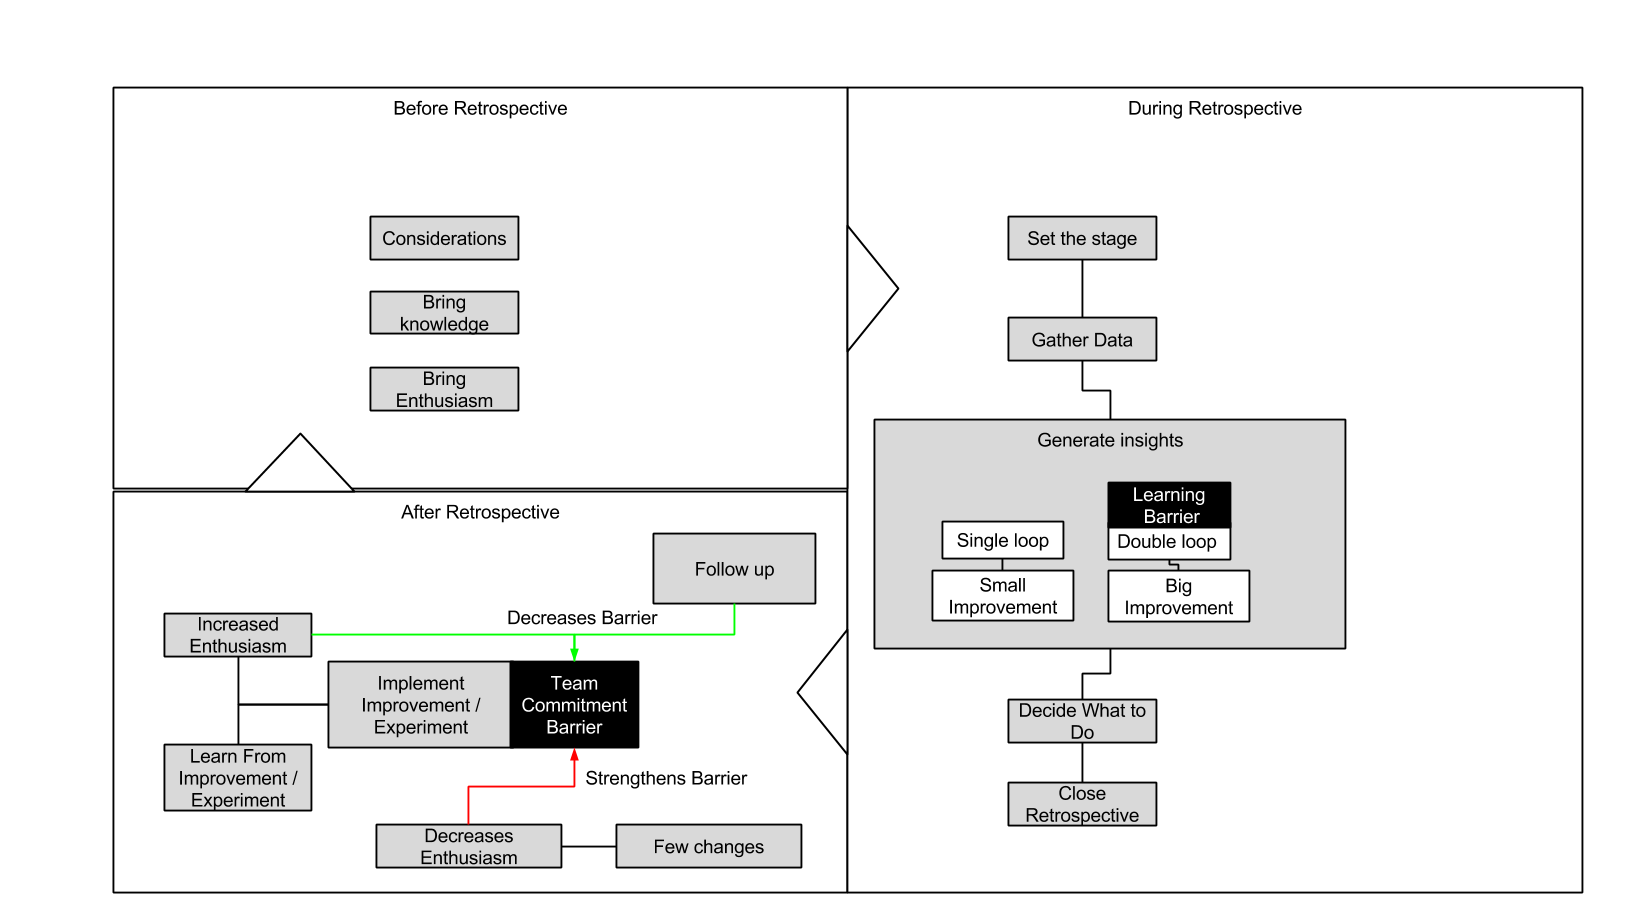
\includegraphics[width=\textwidth, keepaspectratio]{figures/retro-outcome.png}
	\caption{Our perceived state of the retrospective.}
	\label{figure:retro-current-state}
\end{sidewaysfigure}

\afterpage{\clearpage}

\subsubsection{Before Retrospective}
The first part of the retrospective practice consists of three elements that we have been able to see through this study: Considerations, bring knowledge and bring enthusiasm. 

Before the retrospective the facilitator or team is required to bring consider some considerations. Dingsøyr \cite{Dingsoyr2004} proposes several things, however we have seen few of this employed in practice. The considerations we have observed employed by teams today are external facilitator and open or structured discussion. Two of the teams, Echo and Alfa had made the decision to employ an external facilitator. Several of the teams had chosen KJ-Sessions as discussion form, while others just held an open discussion. We have not seen any evidence that any of the teams has made any informed decision on Dingsøyr's considerations. 

Bringing knowledge and enthusiasm is required by the participants before the retrospective. If no one of the 

\subsubsection{During Retrospective}

\subsubsection{After Retrospective}



\subsection{Method Proposal: Meta-Retrospective}
\label{section:Method-propsal}
In this section we aim to discuss the potential of improving the current state of the retrospective in a team. We will propose a method based mainly on our depth study work with team Zulu. This method we decided to call a ``Meta-retrospective''. The intention is to provide a framework for evaluating the current state of a retrospective in a project, and potentially improving the retrospective process as a result. The aim of this process is to decrease the learning barriers affecting the team. An overview figure can be seen in \autoref{figure:retro-meta-state}. This section will describe a process on how a ``Meta-retrospective'' potentially could be conducted.

\paragraph{Motivation for meta-retrospective}
After observing 

\paragraph{Set the stage}
The very first step necessary is to set the stage for the retrospective. This includes informing the team of the intent of the meta-retrospective, making sure that they understand and the focus is long term learning, for example a team member might think that the meta-retrospective will just cover the most recent sprint. A second consideration is who should facilitate the meta-retrospective, in our work with team Zulu we acted as an external facilitator. This was considered a positive aspect by the team leader in, as seen in \autoref{result:learning-reflection-zulu}. However this responsibility should be delegated after consideration by suitable personnel, for example the team leader or SCRUM master. 

\paragraph{Gather data}
The second step for the meta-retrospective is to gather data that will serve as a basis for discussion. This is in order to contribute an objective assessment of the 

\paragraph{Reflect on learning}

\paragraph{Decide what to do}

\paragraph{Decide on future actions} % (fold)
\label{par:paragraph_name}

\paragraph{Close Meta-retrospective} % (fold)
\label{par:paragraph_name}
del i to

% paragraph paragraph_name (end)

% paragraph paragraph_name (end)


\todo[inline]{Skriv og knytt til egne funn}

\begin{sidewaysfigure}[!h]
	\centering
	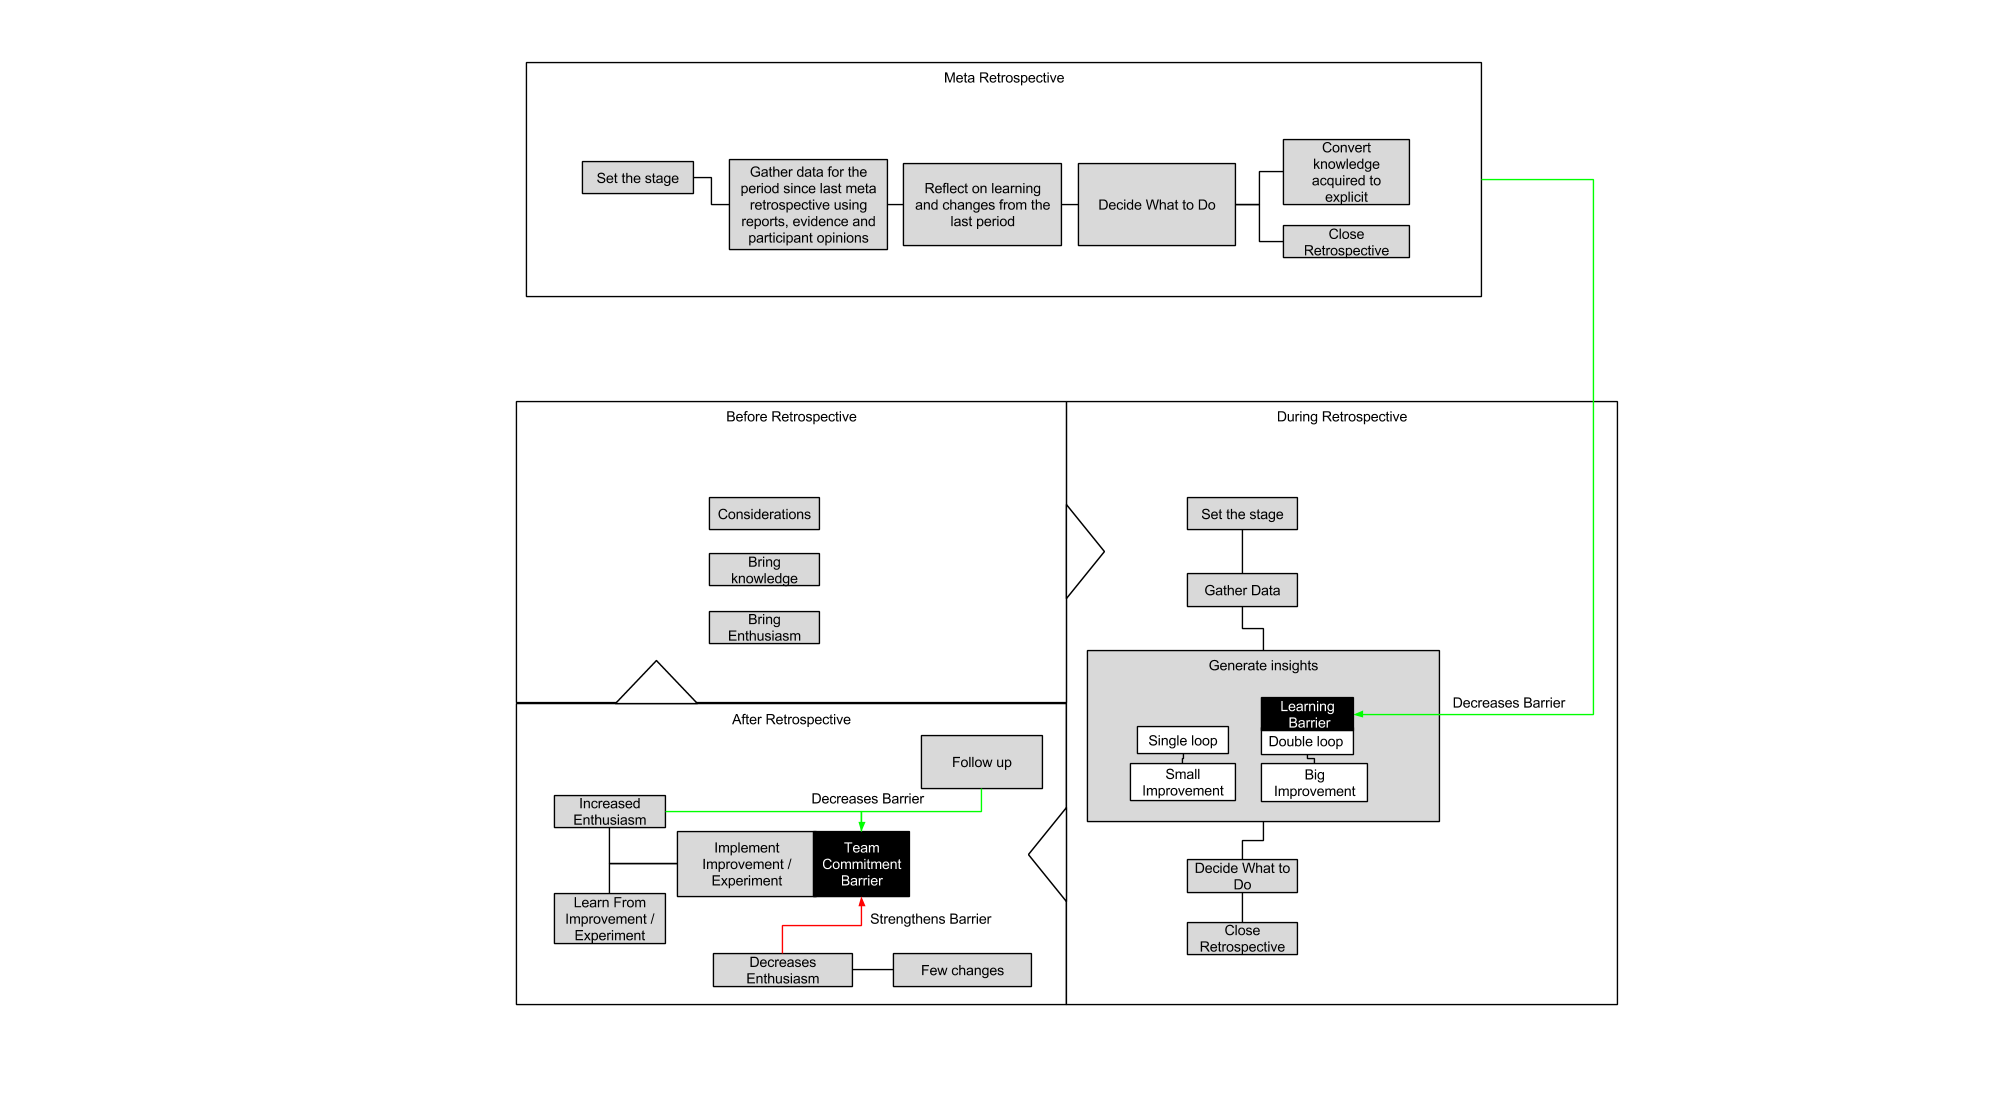
\includegraphics[width=\textwidth, keepaspectratio]{figures/meta-retro.png}
	\caption{Retrospective state after introduction meta-retrospective}
	\label{figure:retro-meta-state}
\end{sidewaysfigure}

\begin{figure}[!h]
	\centering
	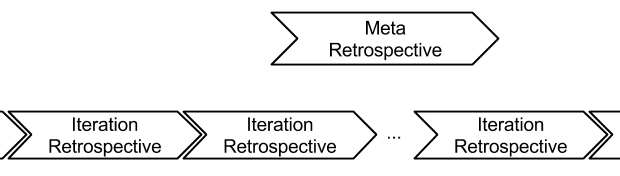
\includegraphics[width=\textwidth, keepaspectratio]{figures/meta-retro-occurence.png}
	\caption{Visualization of meta-retrospective occurrence}
	\label{figure:retro-meta-occurence}
\end{figure}

\subsection{Guidelines for Conducting Retrospectives}

Through this study we have identified several characteristics that we believe will have positive impact on the conduction of the retrospective process in a modern team. These will be presented in a set of guidelines, followed by a short explanation of each point.

\begin{itemize}
	\item External facilitating.
	\item Implementation of actions 
	\item Address actions to name and visualize
	\item Enthusiasm
	\item Trust
	\item Ownership
	\item Experimentation
	\item Reflection on own learning. (link til meta retro)
	\item Regular retrospectives
	\item Measured varying of technique
	\item Find root causes
	\item Follow up implementations
	\item Reflect on how to conduct own retrospective
	\item Move beyond day-to-day decisions
\end{itemize}

\paragraph{External facilitating}
As described in \autoref{section:facilitator} we observed multiple instances in which the use of an external facilitator was positive to the team. There are multiple approaches that could be used to arrange an external facilitator, an example would be switching SCRUM masters between teams in the company, another possibility would be using personnel from outside the company.

\paragraph{Implementation of actions}
The ensuring implementation of actions appears critical for a team to have confidence and trust in the retrospective process. Therefore attempts to conduct a good retrospective should attempt to ensure that actions are completed, and that this success of this is acknowledged by the team. As seen in our work with team Zulu this is very possible and can lead to a positive effect in the team. Implementation of actions feeds the positive loop described in \autoref{section:positive-loop-enthusiasm}.

\paragraph{Address actions to name and visualize}
One step we observed that had a major impact on the implementation of actions was the follow-up protocol. In \autoref{table:follow-up-techique} we observe that the teams assigning name to an action are satisfied with their protocol are satisfied. Another positive step is the visualization of the actions.


\paragraph{Follow up implementations}
A team should ensure that there is some sort of follow up that ensures that actions are implemented. For example this responsibility can fall to SCRUM master as seen in team Echo in \autoref{question-6}.

\paragraph{Trust}
The building of trust seems absolutely central to unlocking the potential of the retrospective session. Thus a team looking to improve should investigate possibilities relating to increasing the sense of trust between team members. One example of the positive impact this can have on a team can be seen in \autoref{question-21}, where team Delta improves team dynamic through a discussion enabled by the high level of trust in the team.

\paragraph{Ownership}
The generation of ownership has a very positive effect on the team's attitude towards retrospective. This is discussed in \autoref{section:positive-loop-enthusiasm}. In order to facilitate this ownership a team should be empowered in their decision making, leading to them shaping their work processes into something they own.

\paragraph{Experimentation}
A retrospective should be open to leading to experimentation. We have observed this lead to several benefits for the teams in our analysis, this is described in more detail in \autoref{section:experiments-in-work-place}. 

\paragraph{Reflection on own learning}
Through our work we discovered that team level reflection on learning processes has little or no presence. The work done with team Zulu indicates that this reflection can provide benefits, and we elaborate our ideas for this characteristic in \autoref{section:Method-propsal}

\paragraph{Regular retrospective}
Teams without regular retrospectives can be negatively affected in several ways, as described in \autoref{section:Retrospective-timespan}. Making sure there is not too long between retrospectives decreases the effect of memory bias as described in \autoref{section:valid-information}.

\paragraph{Measured varying of technique}
We got a wide range of answers when we investigated the use of techniques in a retrospective, as seen in \autoref{section:retrospective-practices-used}. Thus it seems advisable for a team to experiment with using different techniques in order to discover what works for them. One should be mindful of too much variation, as too much variation could steer focus over to the technique instead of the retrospective session

\paragraph{Reflect on how to conduct own retrospective} % (fold)
A team can improve by reflecting how they can benefit from established theory, for example considering how they compare to Dingsøyr's approach elaborated on in \autoref{section:Dingsoyr-Approach-Introduction}.


\paragraph{Find root causes}
As described in \autoref{discussion:learning-impediments} some teams can benefit from increasing their focus on double-loop learning. This can lead to more effective decision making as underlying issues are targeted instead of superficial ones. Some techniques observed to find root causes are described in section \autoref{question-13}.

\paragraph{Move beyond day-to-day decisions}
Our work has seen that a retrospective have a potential to move beyond operational decisions, this is for example shown in \autoref{section:decision-making-zulu}. A team mindful of this potential is better suited to improve from their retrospective.


 
\subsection{Future Work}

\paragraph{Expansion on shared mental models}


\clearpage
